%%%%%%%%%%%%%%%%%%%%%%%%%%%%%%%%%%%%%%%%%%%%%%%%%%%%%%%%%%%%%%%%%%%%%%%%%%%%%%%%%%%%%%%%%%%%%%%%%%%%%%%%%%%%%%%%%%%%%%%%%%%%%%%%%%%%%%%%%%%%%%%%%%%%%%%%%%%%%%%%%%%
% Written By Michael Brodskiy
% Class: Electricity & Magnetism
% Professor: D. Wood
%%%%%%%%%%%%%%%%%%%%%%%%%%%%%%%%%%%%%%%%%%%%%%%%%%%%%%%%%%%%%%%%%%%%%%%%%%%%%%%%%%%%%%%%%%%%%%%%%%%%%%%%%%%%%%%%%%%%%%%%%%%%%%%%%%%%%%%%%%%%%%%%%%%%%%%%%%%%%%%%%%%

\documentclass[12pt]{article} 
\usepackage{alphalph}
\usepackage[utf8]{inputenc}
\usepackage[russian,english]{babel}
\usepackage{titling}
\usepackage{amsmath}
\usepackage{graphicx}
\usepackage{enumitem}
\usepackage{amssymb}
\usepackage[super]{nth}
\usepackage{everysel}
\usepackage{ragged2e}
\usepackage{geometry}
\usepackage{multicol}
\usepackage{fancyhdr}
\usepackage{cancel}
\usepackage{siunitx}
\usepackage{physics}
\usepackage{tikz}
\usepackage{mathdots}
\usepackage{yhmath}
\usepackage{cancel}
\usepackage{color}
\usepackage{array}
\usepackage{multirow}
\usepackage{gensymb}
\usepackage{tabularx}
\usepackage{extarrows}
\usepackage{booktabs}
\usepackage{lastpage}
\usetikzlibrary{fadings}
\usetikzlibrary{patterns}
\usetikzlibrary{shadows.blur}
\usetikzlibrary{shapes}

\geometry{top=1.0in,bottom=1.0in,left=1.0in,right=1.0in}
\newcommand{\subtitle}[1]{%
  \posttitle{%
    \par\end{center}
    \begin{center}\large#1\end{center}
    \vskip0.5em}%

}
\usepackage{hyperref}
\hypersetup{
colorlinks=true,
linkcolor=blue,
filecolor=magenta,      
urlcolor=blue,
citecolor=blue,
}


\title{Homework 2}
\date{September 28, 2023}
\author{Michael Brodskiy\\ \small Professor: D. Wood}

\begin{document}

\maketitle

\begin{enumerate}

  \item Six charges are arranged along the sides and corners of a square with sides of length L as shown. Calculate the magnitude and direction of the electric field at the origin. Use symmetry and superposition to make the calculation simple.

    \begin{center}
      \begin{figure}[h]
        \centering
        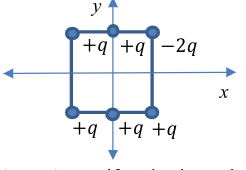
\includegraphics[width=.4\textwidth]{Figures/Figure2-1.png}
        \label{fig:1}
      \end{figure}
    \end{center}
    
  \item A uniformly charged rod of length $L$ and charge $q$ is placed along the $x$-axis with its center at $x=a$. Find the $x$-component of the electric field at a point on the $z$ axis. (Hint: use $R$ as the variable of integration.) Check your expression in the following limit: $z=0$ and $a>>L$.

    \begin{center}
      \begin{figure}[h]
        \centering
        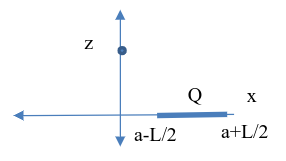
\includegraphics[width=.4\textwidth]{Figures/Figure2-2.png}
        \label{fig:2}
      \end{figure}
    \end{center}
    
  \item Calculate the electric potential on the $z$-axis due to a uniformly charged annulus in the $xy$-plane centered at the origin with inner radius $a$ and outer radius $b$. Then find the electric field from the gradient of the potential.
    
  \item Consider an infinitely long uniformly-charged solid cylinder of radius $a$ and charge per unit volume $\rho$ surrounded by a coaxial cylindrical shell of radius $b$ and charge per unit area of $\sigma$. Take the axis of the cylinders as the $z$-axis.

    \begin{enumerate}

      \item Calculate the electric field everywhere in space

      \item Also calculate the potential as a function of the distance from the axis, taking the potential to be zero on the $z$-axis.

    \end{enumerate}
    
  \item The electric field for two charged concentric spherical shells is given by

    $$\left\{\begin{array}{c c} 0, & r<a\\ \bold{\hat{r}}A_1/r^2, & a< r< b\\ \bold{\hat{r}}A_2/r^2, & r>b \end{array}$$

      Where $A_1=5\times 10^6\left[ \frac{\si{\newton\meter\squared}}{\si{\coulomb}} \right]$, $A_2=-3\times10^6\left[ \frac{\si{\newton\meter\squared}}{\si{\coulomb}} \right]$, $a=.25[\si{\meter}]$, and $b=.45[\si{\meter}]$. Find the surface charge densities $\sigma_a$ and $\sigma_b$ on the two shells.
    
\end{enumerate}

\end{document}

